\documentclass[authoryear, 12pt,5p, times]{elsarticle}
\usepackage[hypcap]{caption}
\usepackage{float}
\usepackage{amsmath}
\usepackage[hidelinks]{hyperref} 
 \usepackage{gensymb}
\usepackage{subcaption}
\usepackage{url}
%\renewcommand\thefootnote{\fnsymbol{\dagger}}
\usepackage[symbol*]{footmisc}
\begin{document}
%\footnote{This is a footnote}
\begin{frontmatter}
\title{Photon Counting \& the Statistics of Light}
\author{\today \\ \quad \\Jung Lin (Doris) Lee\\ dorislee@berkeley.edu\\Group partners: Jennifer Ito, Manuel Silvia\\Prof. James Graham, UGSI Heechan Yuk, Isaac Domagalski}
	\begin{abstract}
    %key objective, method, principle conclusion 
	  In our experimental setup, photons emmited by an LED light source is regestered by the PMT as a timestamp for every photon detection. By increasing the brightness of the light source, we found that photon arrival rates increase. Analysis on a single dataset shows that as the the number of events in an experiment (N) increases, the sample mean($\bar{x}$) converges to the theoretical mean($\mu$).  The fluctuation around this value of $\mu$ falls off as with 1/$\sqrt{N}$, so increasing N can results in more reliable experimental results. However, systematic effects can not be eliminated by such methods. We instead mitigate the afterpulsing effect by vetoing events that occurred immediately after another. The processed data results in a histogram that align very closely to exponential distribution. In addition, binned data for a fixed time interval also matches closely with the Poisson distribution. Finally, we can obtain the sample mean parameter for this  experiment by fitting the histogram to the Poisson distribution.  
	\end{abstract}
\end{frontmatter}
\section{Introduction\label{intro}}
\indent Large sky surveys such as the Sloan Digital Sky Survey(SDSS) and the Dark Energy Survey (DES) have surveyed large fractions of the sky providing detailed photometric and astrometric information for millions of sources. Much like how photons from an LED arrive at the PMT in our experiment, images are formed by individual photons that reaches the CCD.  Therefore, some of the surveys' calibration pipeline relies on the knowledge of photon statistics, as  they are governed by the same set of underlying noise and distribution. An understanding of how these systematic may affect the imaging data may be helpful in studying individual galaxy morphology, determining the transit of an exoplanet, or compiling brightness-limited catalogs for cosmological studies.  
 \\
\indent In this report, we present the methods used to conduct the photon counting experiment and the obtained statistical results. In section \ref{experiment}, I will detail the experimental method that my group used to take the data. Then, section \ref{stats} introduces the various statistical measures that were used to describe the findings on a single dataset. Section \ref{pstats} introduces the two probability density functions (PDFs) dthat are relevant to the histograms of these datasets.
\section{Experiments\label{experiment}}
	\subsection{Methods}
\indent In the setup, the light from the LED is directed into a optical fiber into the photomultiplier tube (PMT) to minimize losses. A squawker and oscilloscope is connected to provide audio and visual feedback for a photon detection. The arrival of a photon is registered by a PMT, and data was acquired using the CoinPro software. The resulting data file is a series of timestamps corresponding to when the photon arrived. Since the CoinPro software is ran on a 32-bit machine, we can see the counts cycling through of time, with the extrema corresponding to the maximum and minimum 32-bit signed integer. Although absolute timestamp is the recorded quantity, it is often more useful to consider the time elapsed between two consecutive events ($\texttt{dt}$) as plotted in Fig.\ref{scatterplot} in order to get a sense of  the photon arrival rate for some period of waiting time.
\begin{figure}[h]
\centering
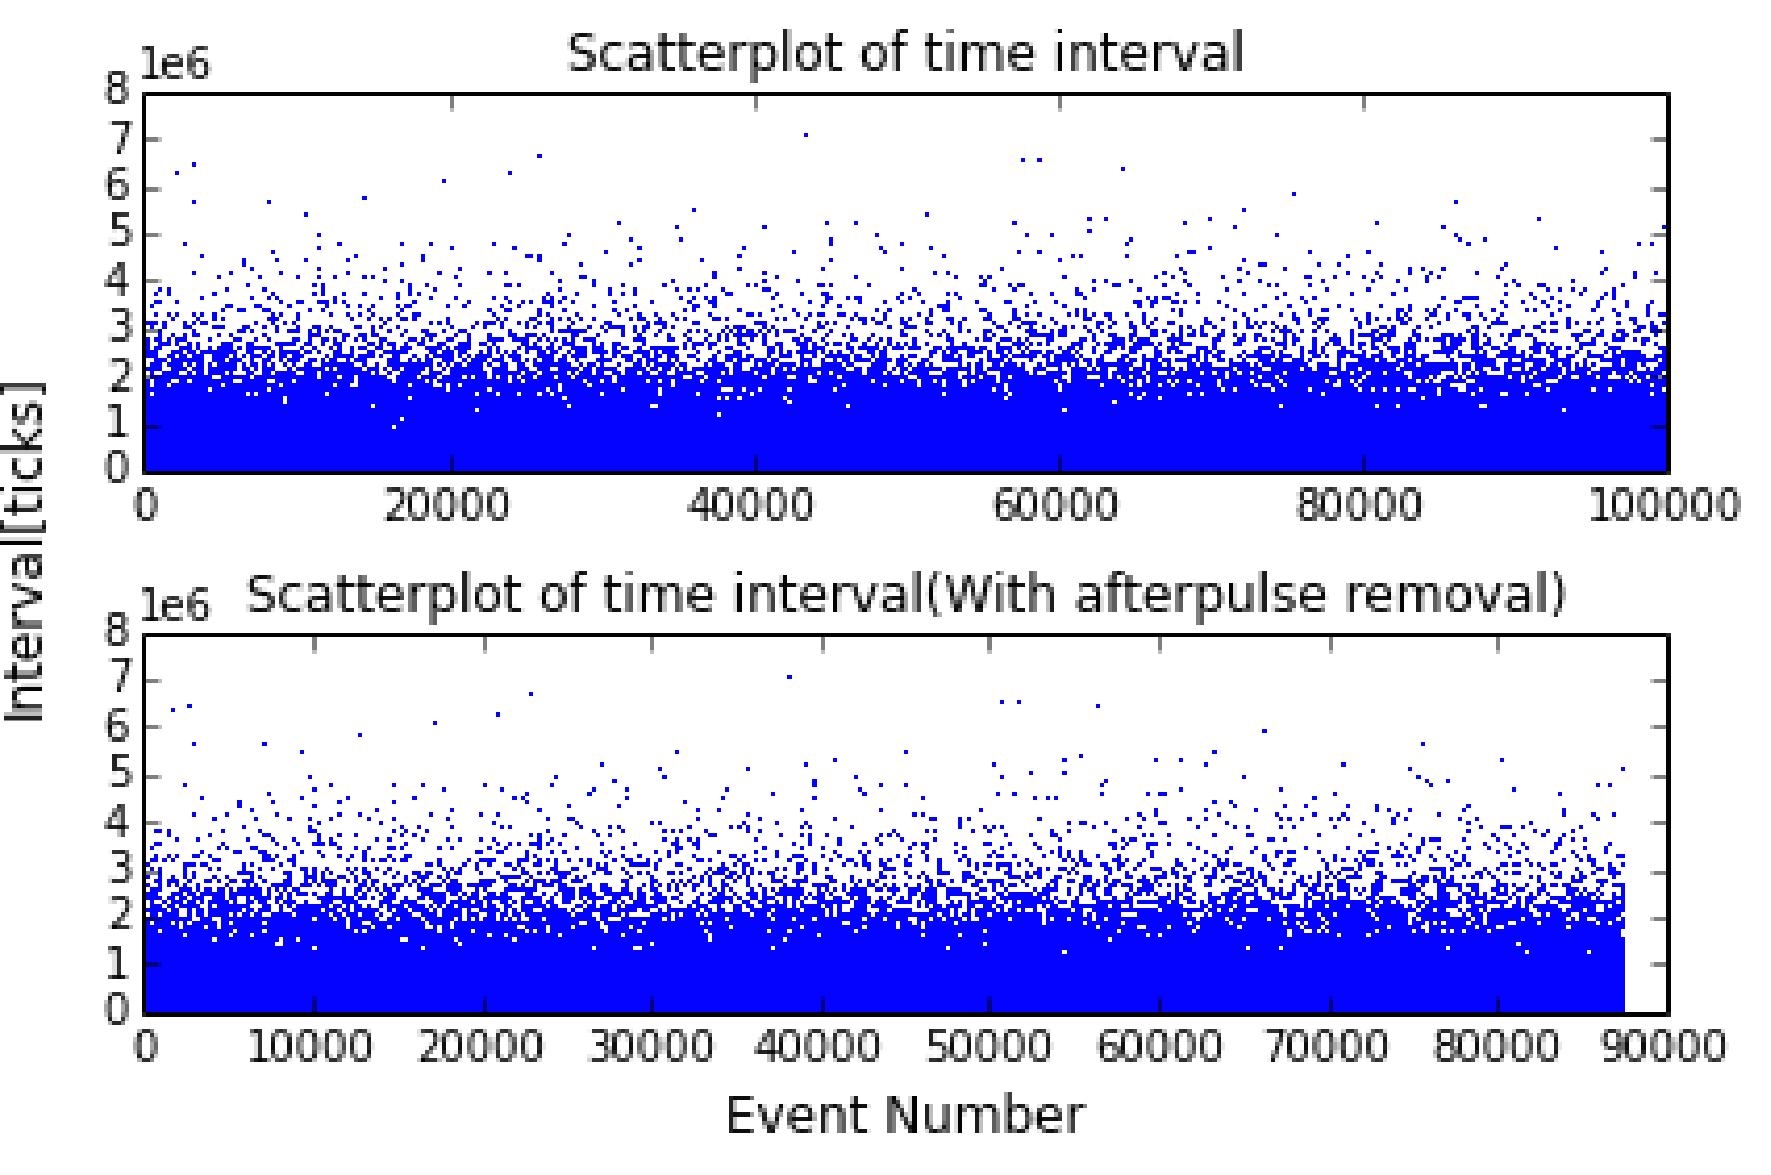
\includegraphics[width=0.5\textwidth]{figures/interval_scatterplot_subplot}
\caption{With the removal of after pulse events, we can see that there is a decline in the number of events. This makes sense because the afterpulse removal procedure cuts away all the interval that lasts 3000 clock ticks or less. As a result of this cut, we expect to see a clear boundary at y=3000, but, due to the large range of interval value that the y-axis spans over, this can not be seen. The data representation in Fig.\ref{changeLED} and \ref{fitted_histo_gate_or_no} better shows the the effect of gating afterpulses. }
\label{scatterplot}
\end{figure}
\\
\indent Sometimes noise pulses resembling Fig.\ref{afterpulse} can be observed after the original pulse. These events are caused by  the ionization of residual gas molecules in the PMT's vacuum chamber.  We eliminate this systematic effect by cutting away data with subsequent pulses lying within the time frame of 2.5$\mu$s  after an original pulse as shown in Fig.\ref{scatterplot}.

\begin{figure}[h]
\centering
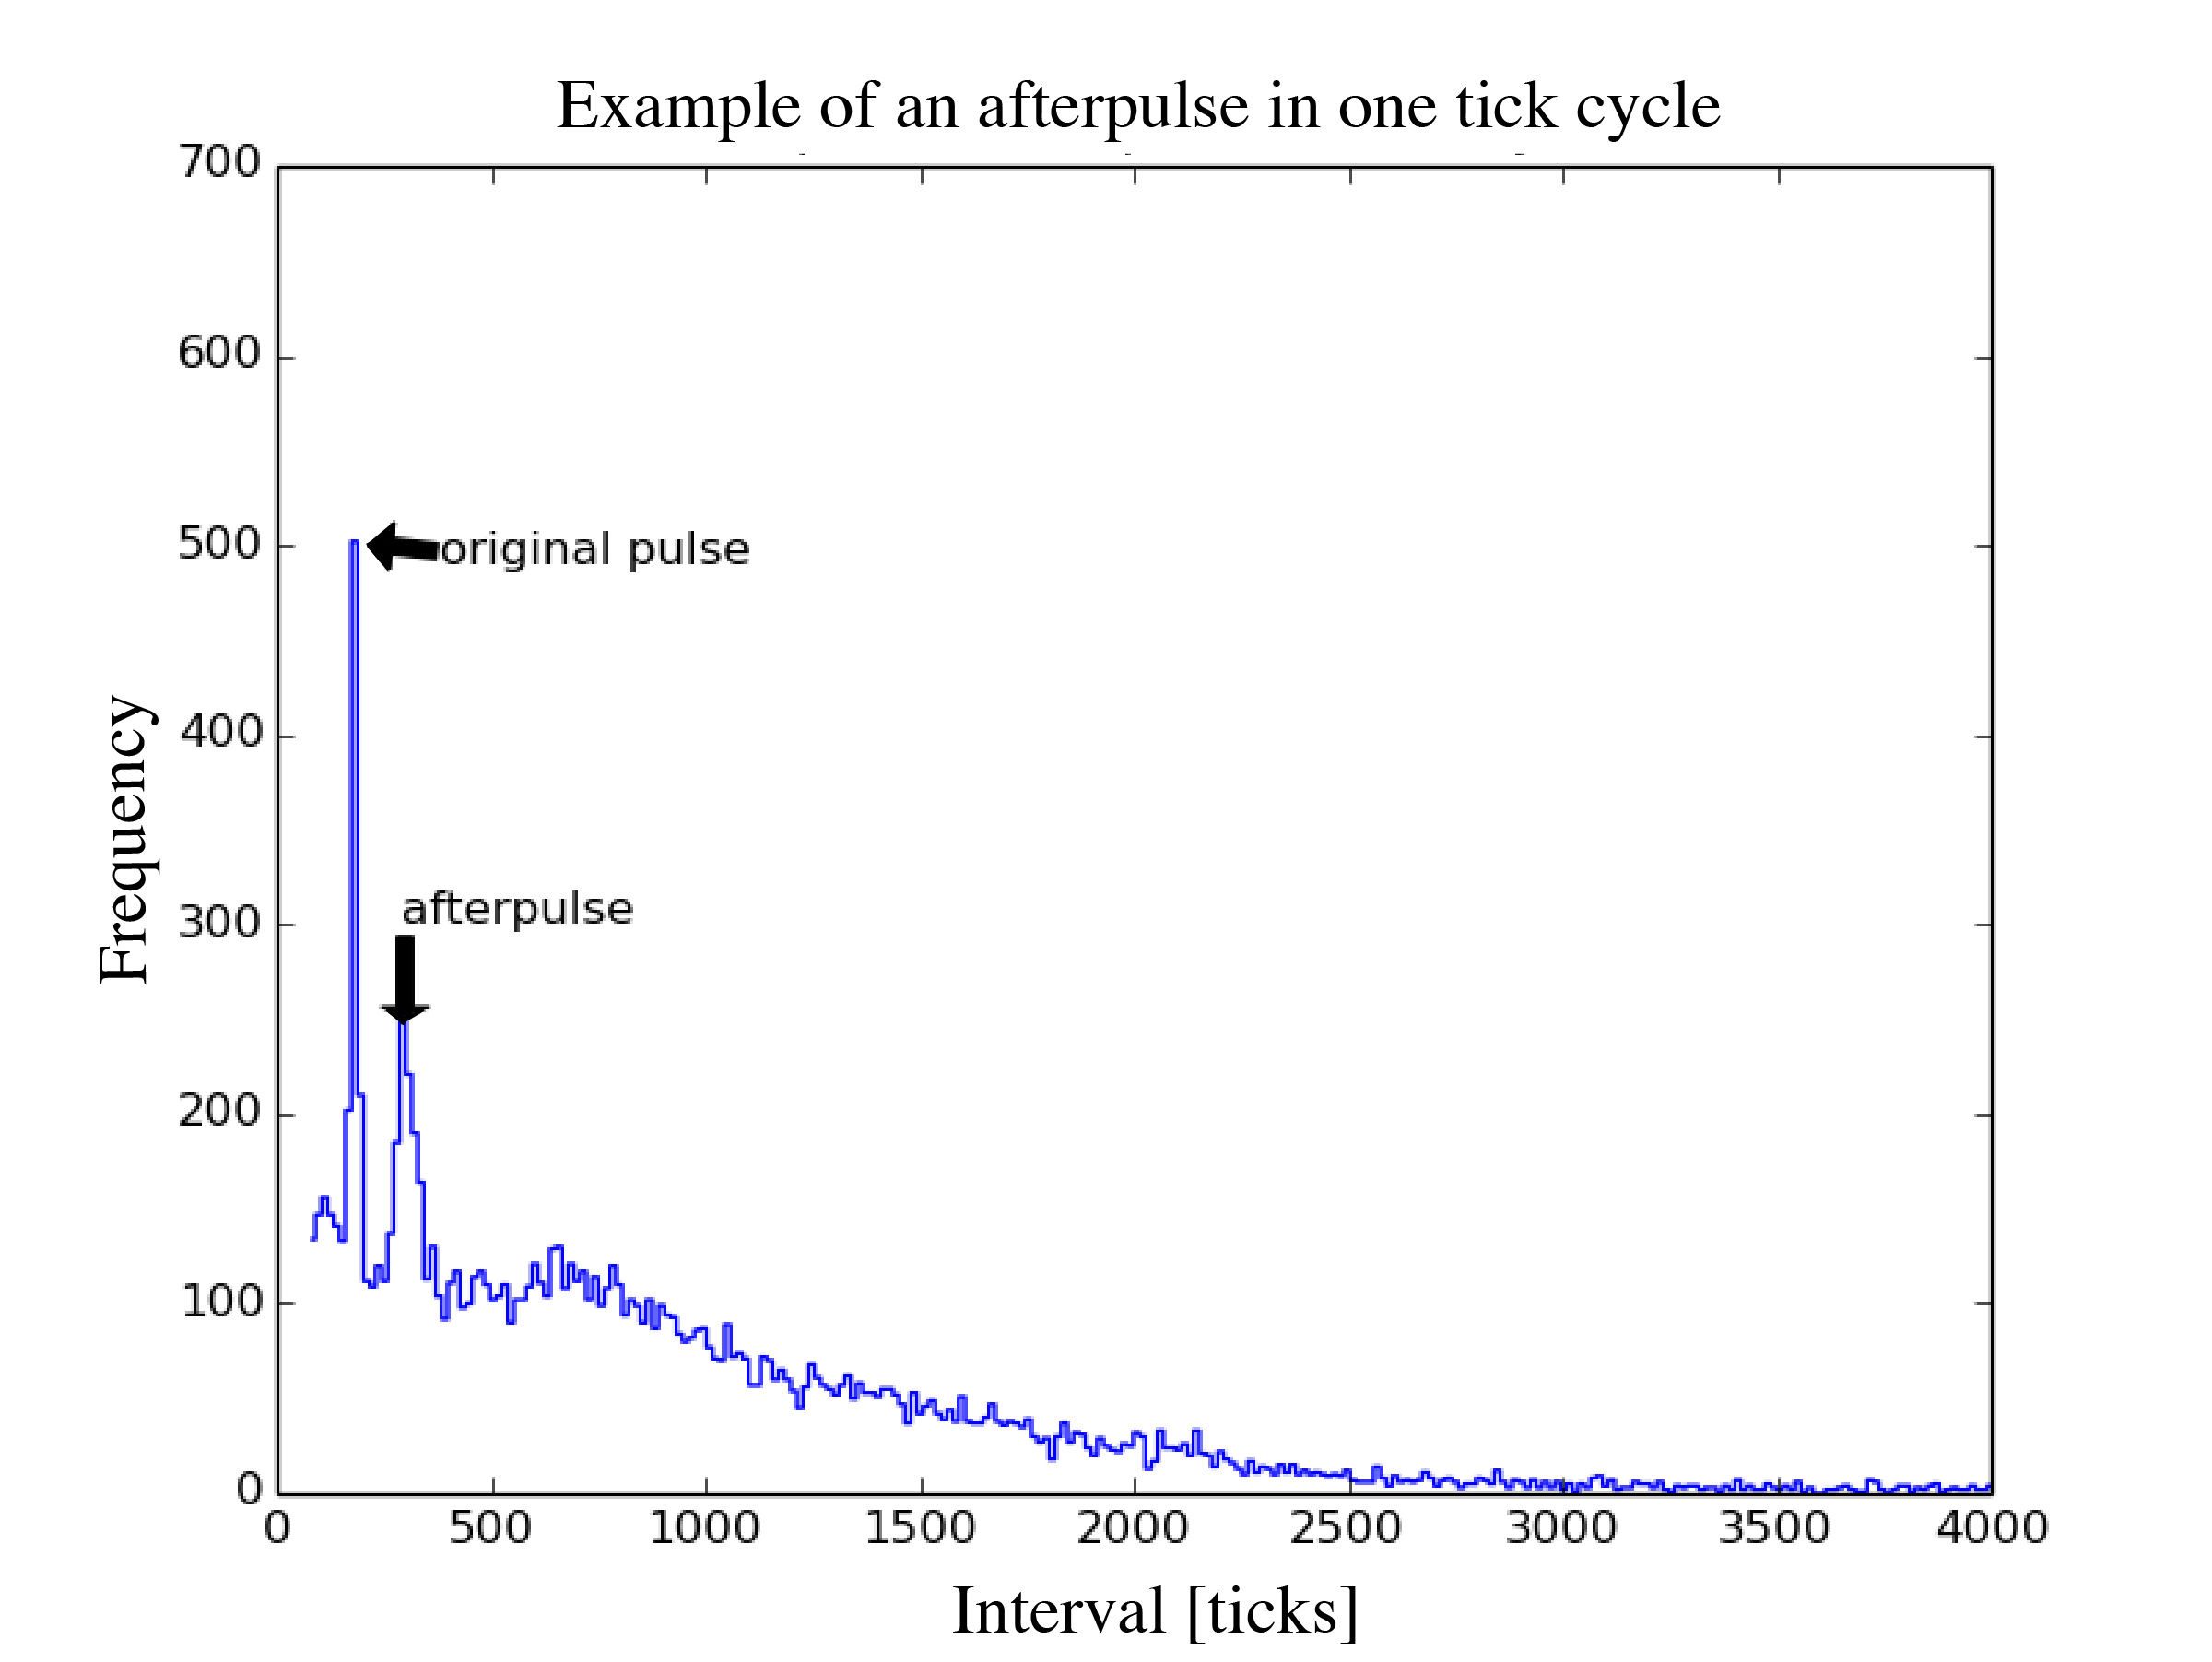
\includegraphics[width=0.5\textwidth]{figures/afterpulse}
\caption{With a histogram of bin size = 500,000, the two peaks (original and afterpulse) as well as a gradual decline of ticks in the next 3000 clock ticks can be seen here.}
\label{afterpulse}
\end{figure}
   \subsection{Changing LED Brightness\label{changeLEDbrightness}}
\indent In order to take a set of data with different brightness level, we listened to ticks on the squawker and found that there was no detectable difference from the 3 o'clock off position to the 12 o'clock position of the LED brightness knob. Therefore, we started off at the 12 o'clock location and went to the max location (at around 90\degree), diving this region into 5 equal parts for the 6 brightness settings\footnote{Although it seems like only 5 data points are shown in the plot, this is merely an artifact of the choice of data representation as circles as  the first two data points lie so closely that they are almost indistinguishable. This is easily verified by using the point representation with \texttt{matplotlib's} `,`setting} of roughly 18\degree  increments. Even though these measurements of the LED brightness were only estimated, it did not significantly affect the plot since the data points should fall on the $\sigma=\bar{x}$ line as the $\sigma$ and $\mu$ of an exponential distribution are always equal.
\begin{table}
    \center
    \begin{tabular}{l|l}
    Intensity[\degree] & Final timestamp in time series [ticks] \\ \hline
    0                                    & 86447071309                                     \\
    18                                   & 68475846523                                     \\
    36                                   & 35127973096                                     \\
    54                                   & 7517634481                                      \\
    72                                   & 5787954870                                      \\
    90 (max)                             & 5558407093                                      \\
    \end{tabular}
    \caption{Intensity is specified as the LED control knob position in degrees, as described earlier in Sec.\ref{changeLEDbrightness}. Since we are taking a fixed number of photon arrival events, as the brightness increases, the faster photon arrival rate means that 10,000 event count finishes faster than it did for lower brightness; thus, accounting for the smaller final  timestamp values.}
    \label{table}
\end{table}
\begin{figure}[h]
%Last timestamp in the reconstructed time series
\centering
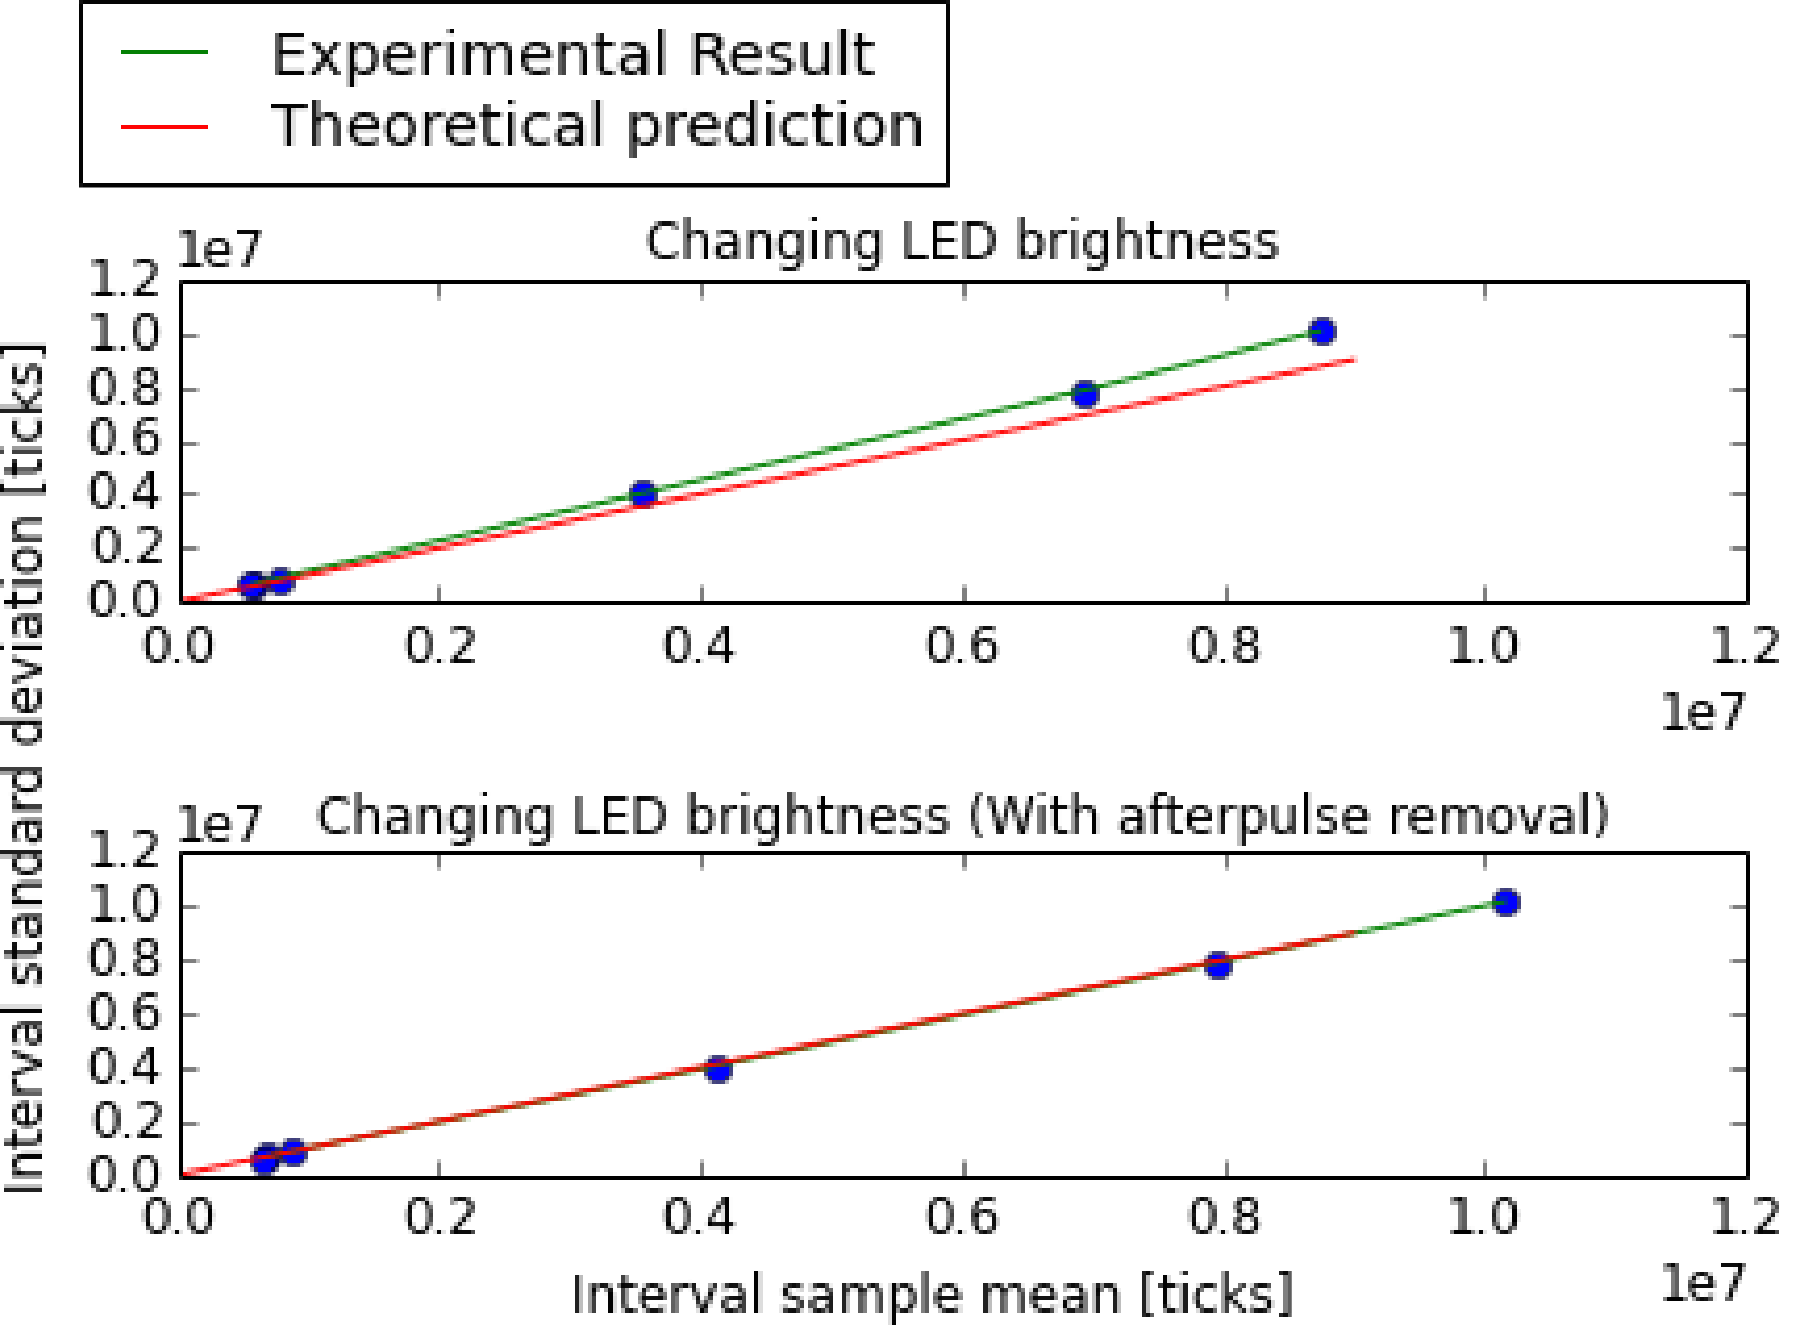
\includegraphics[width=0.5\textwidth]{figures/changeLED}
%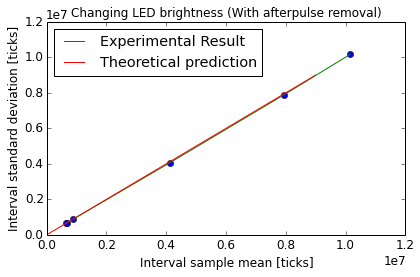
\includegraphics[width=0.5\textwidth]{figures/changeLED_gating}
\caption{The slope of the line should be one since both the standard deviation and the sample mean of each dataset is equal to the single-parameter $\tau$ in the exponential distribution. We find that gating the afterpulses causes the $\bar{x}$ to get closer to $\mu$. }
\label{changeLED}
\end{figure}
\section{Descriptive Statistics\label{stats}}
\subsection{Simple Descriptions of Data}
Using the largest dataset we collected with the LED on maximum brightness, we obtain a sample mean of 561571 ticks and a standard deviation of  637988 ticks on the whole dataset of 99833 events.\footnote{CoinPro does not stop the event count at exactly 100,000 events.} This is the most precise statistical quantity we can obtain using our largest dataset, since the more data that we compute with the closer the sample mean converges to the mean value as shown in Fig.\ref{stat_converging}. Although higher precision measurement of $\bar{x} $ and $\sigma$ can be obtained by taking a sample of larger N so that $\bar{x}$ approaches $\mu$, but this does not ameliorate any systematic effect such as dark current or afterpulses.
 	\begin{figure}[h]
		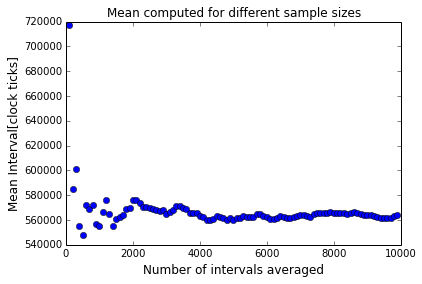
\includegraphics[width=0.5\textwidth]{figures/converging_mean}
		\caption{Large fluctuation in computed mean decreases as larger datasets are used to compute the mean.}
		\label{stat_converging}
	\end{figure}
	\subsection{Standard Deviation of the Mean (SDOM)}
		The SDOM tells us the uncertainty on the sample mean obtained from the given set of N datapoints. The 1/$\sqrt{N}$ behavior shown in Fig.\ref{sdom} is important since it motivates an experiment with greater number of events, as it increases the confidence level in the experimental results.
	 	\begin{figure}[ht]
		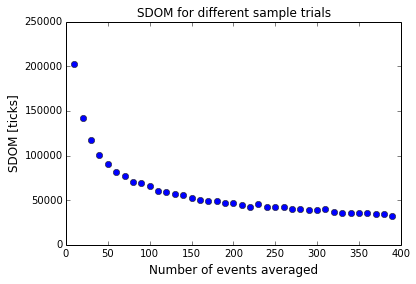
\includegraphics[width=0.5\textwidth]{figures/sdom_exp_graph}
		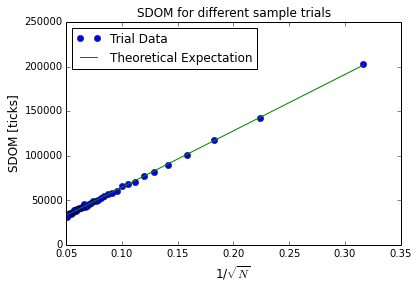
\includegraphics[width=0.5\textwidth]{figures/sdom_linear}
		\caption{The top graph shows how SDOM declines as a function of the number of events. The resulting curve resembles an inverse-root relation. We test this hypothesis by transforming the x-axis into 1/$\sqrt{N}$ and we indeed observe a linear relationship with the sample standard deviation as the slope.}
		\label{sdom}
	\end{figure}
\section{Photon Statistics\label{pstats}}
Even though mean and standard deviation are useful descriptive quantities that characterizes the data, they are actually properties of the underlying distribution. Despite the inevitable loss of details from the binning procedure, histograms can often provide additional information about the distribution of data. In this section, I will explain how different types of binning leads to the exponential and Poisson distribution and how they are related. 
 	\subsection{Exponential Distribution}
 	Exponential distribution described by Eq.\ref{exp_distr} governs the histogram of the elapsed time between photon arrival event ($\texttt{dt}$).
\begin{align} 
P(t,\tau)=\frac{1}{\tau}e^{-\frac{t}{\tau}}
\end{align}
\\where  $\Delta t= $time step-size and  $\tau=$mean interval.
\\  A defining characteristic of the exponential distribution is that it is continuous``memorylessness``: photon arrival rate at some moment in time,t, is not dependent on the photon arrival rate prior to time t.  The green curve in Fig.\ref{fitted_histo_gate_or_no} is the plotted from the analytical solution shown in Eq.\ref{int_exp}. This result is obtained from integrating the exponential distribution with a  $\Delta t =1.42\times10^7$ and $\tau$ set as the mean of the $\texttt{dt}$ dataset .  
 	 \begin{equation}\label{int_exp}
 	 \int^{t+\Delta t}_\tau\frac{1}{\tau}e^\frac{t}{\tau}dt=-e^\frac{t+\Delta t}{\tau}+e^\frac{t}{\tau}
	\end{equation} 	  
Since the exponential PDF is normalized to one, this result is scaled by the number of events to fit the histogram.
 	\begin{figure}[h]
		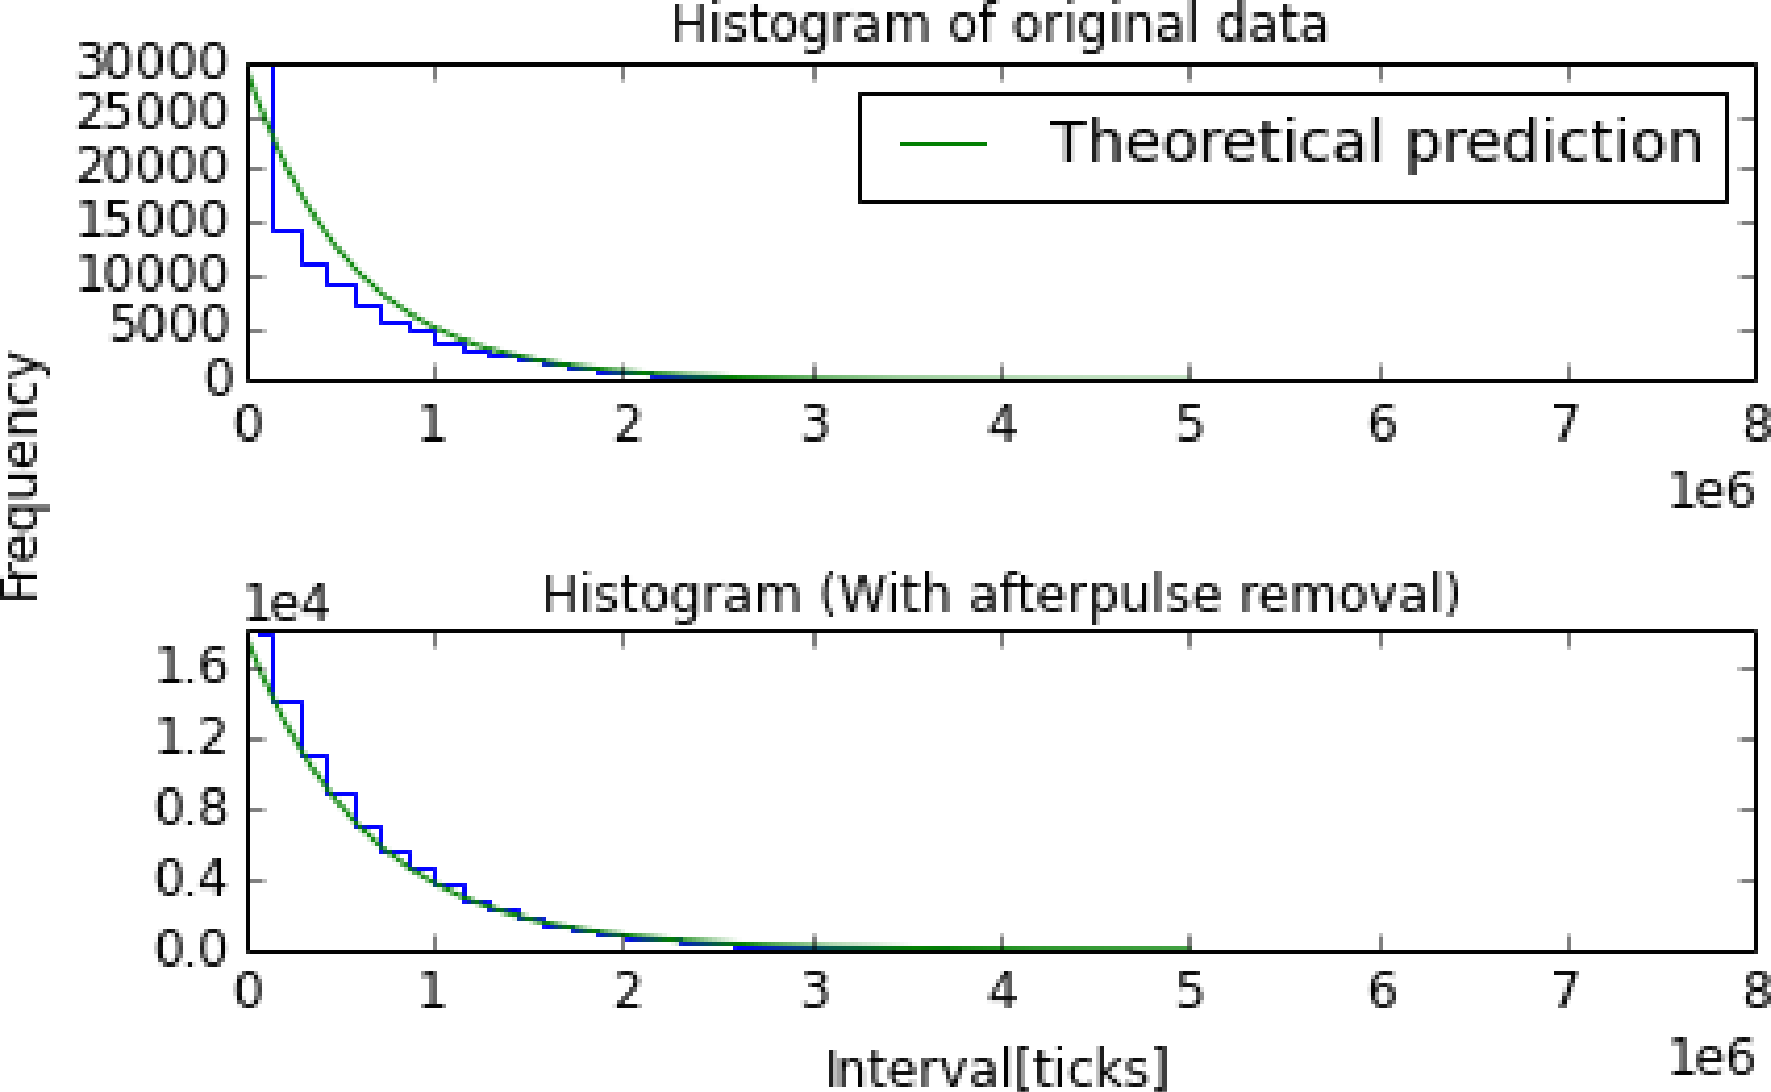
\includegraphics[width=0.5\textwidth]{figures/histogram}
		\caption{A histogram of bin size of 50 before and after gating afterpulses, with the scaled exponential PDF fit. Note that the histogram fits closer to the exponential distribution after the afterpulse removal.}
		\label{fitted_histo_gate_or_no}
	\end{figure}
 	\subsection{Poisson Distribution}
 	Although closely-related, the Poisson distribution is unlike the exponential distribution in that it is a discrete probability distribution that arises from measuring the number of events that occur within a fixed sampling interval. Both underlying process applies to rare event for very large N, but the experiment method is different. In this case, the experiment is the same, but we change the way the data is represented, as binned data for a fixed time interval.
 	 	\begin{figure}[h]
			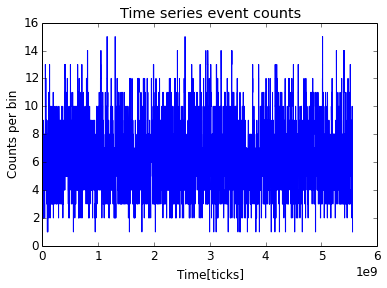
\includegraphics[width=0.5\textwidth]{figures/time_series}
			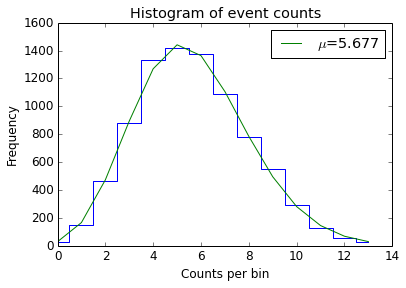
\includegraphics[width=0.5\textwidth]{figures/poisson_histo}
			\caption{The bin counts are obtained by counting the number of photon arrival events that lie within an interval of 3.09 milliseconds. From the time series plot, we see that most time intervals counted 4 to 8 events. This is confirmed by using a Poisson curve fit on the histogram where the value of the fitting parameter is 5.677.}
			\label{poisson}
		\end{figure}
\section{Conclusion\label{end}}
In this experiment, the apparatus is setup such that the PMT registers the photons emitted by the LED light source and the timestamp is recorded by the CoinPro program.  We found that by changing the brightness of the light source, the photon arrival rate increases, resulting in a shorter time series. By analyzing the interval between subsequent events, we observe interesting statistical properties that governs the datasets. \\ \indent Since photon arrival is rare, random, and in the limit of large N, the mean interval histogram resemble closely to a exponential distribution. By binning the data with a fixed interval width and fitting a Poisson distribution over the resulting histogram, we can get the value of the $\bar{x}$ parameter.  The Poissonian fluctuations in the photon arrival timing are yields an uncertainty of $\sqrt{N}$. Such fluctuations are random and independent of any systematic error. Therefore, we can not use the approach of increasing N to mitigate the afterpulse effect. Instead, we vetoed  spurious ion events that followed immediately after a real photon emission and obtained more accurate results.
\\ \indent As we only attempt to mitigate the effect of one type of systematic error, one possible extensions to this project may be to investigate the effect of other types of systematic error such as dark counts and read noise on the quality of the data. This effect can be quantified by measuring the signal to noise ratio and comparisons among different types/manufacturers of PMTs.
\section{References}
\footnotesize
Pickett, Siobhan, Sean Carriedo, and Chang Wang. ``Determining the Signal-to-Noise Ratio and Optimal Photomultiplier Gain Setting in the GenePix 4000B." \textit{Genomics Application Note} (2001)
\end{document}
